% ----------------------------------------------------------------------------
% Copyright (c) 2016 by Burkhardt Renz. All rights reserved.
% Die Vorlage für eine Abschlussarbeit in der Informatik am Fachbereich
% MNI der THM ist lizenziert unter einer Creative Commons
% Namensnennung-Nicht kommerziell 4.0 International Lizenz.
%
% Id:$
% ----------------------------------------------------------------------------

\chapter{Themenüberblick}
\label{chapter:Themenüberblick}

\section{Verteilte Systeme}
\label{section:Verteilte Systeme}

Verteilte Systeme dienen als Anwendungsfeld für die Instrumentalisierungsbibliothek. Auch das in dieser Arbeit vorgestellte Testbett ist ein solches verteiltes System. Dazu ist es wichtig,  verschiedene Eigenschaften und Konzepte von verteilten Systemen zu definieren. Diese Eigenschaften und Konzepte nehmen einen entscheidenden Faktor bei der Ermittlung, Analyse und Umsetzung von Anforderungen der Instrumentalisierungsbibliothek ein. Dementsprechenend wird zunächt der Begriff des verteilten Systems definiert:

\begin{quote}
	Ein verteiltes System ist eine Kollektion unabhängiger Computer, die den Benutzern als ein Einzelcomputer erscheinen\footpartcite{10.5555/1202502} 
\end{quote}

\subsection{Eigenschaften eines verteilten Systems}
\label{subsection:Eigenschaften eines verteilten Systems}
	Die Definition von van Steen und Tanenbaum geht mit zwei charakteristischen Eigenschaften von verteilten Systemen einher. Die erste Eigenschaft äußert sich darin, dass alle Komponenten eines Systems unabhängig voneinander agieren können. Komponenten werden in diesem Zusammenhang auch Knoten genannt. Knoten sind Hardwarekomponenten, also pysikalische Recheneinheiten. Auch Prozesse innerhalb einer Hardwareeinheit können Knoten sein. Dabei ist es möglich, dass mehrere Knoten auf einer Hardwareheinheit sind.\footpartcite[p. 2]{VanSteen2017}.

	Knoten sind miteinandern über Netzwerke verknüpft. Innerhalb des Netzwerk kommunizieren Knoten mittels Nachrichten miteinander. Beim Ansprechen eines verteilten Systems soll dem Anfragesteller, zum Beispiel ein Client eines Webservers, nicht ersichtlich sein, dass mehrere Komponenten ein Gesamtsystem bilden, welches die Anfrage verarbeitet und entsprechende Vorgänge ausführt. 
\subsection{Beobachtbarkeit von verteilten Systemen}
\label{subsection:Beobachtbarkeit von verteilten Systemen}
	Unter Beobachtbarkeit versteht man die Möglichkeiten der Betrachtung eines System. Die Symptome, die entstehen können, falls unerwünschte oder unvorhergesehene Zustände in dem System entstehen, sind oft schwer nachvollziehbar. Speziell verteilte Systeme erschweren die Reproduktion solcher Symptome, da das komplexe ineinandergreifen der Komponenten die Erfassung der Vorgänge erschweren. 

	Die Beobachtbarkeit von verteilten Systemen kann in erster Linie durch Überwachung diverser Komponenten des Systems ermöglicht werden. Dabei lassen sich diese Komponenten in drei Kategorien unterteilen. Aufzuzählen sind (\lowroman{1}) \textbf{Hardware} auf denen die Knoten angesiedelt sind, (\lowroman{2}) \textbf{Netwerke}, in denen die Kommunikation der einzelnen Knoten stattfindent und die (\lowroman{3}) \textbf{Anwendung}, welches sich auf alle Knoten verteilten kann.

	
	\textbf{Hardware}\space\space\space Aufgrund der vielzahl an Hardwarekomponenten in einem System gilt es, besonders interessante Komponenten, im Kontext der Fehlerfindung beziehungsweise der Performanceanalyse, zu beobachten. Als Hauptkomponenten der meisten Systeme zählen zum Beispiel die \emph{\gls{cpuLabel}}, die \emph{\gls{gpuLabel}} oder auch die verschiedenen Speicher wie zum Beispiel der \emph{\gls{ramLabel}} oder die \emph{\gls{hddLabel}}. Aus der Beobachtung dieser Komponeten gewinnt man allgemeine Informationen über das Gesamtsystem. Diese Informationen können zum Beispiel dazu genutzt werden, die Auslastung einzelner Knoten zu ermitteln und eventuell auf unbalancierte Nutzung der Konten reagieren zu können oder auftretende \emph{bottlenecks}, das heißt stark auffällige performancebeeinträchtigende Komponenten im System, erkennen zu können. Diese könnten beispielsweise langsame HDDs sein, auf die oft zugegriffen wird.
	
	\textbf{Netzwerk}\space\space\space Die Kommunikation innerhalb des Systems wird durch das Netzwerk, also die Verknüpfung der jeweiligen Knoten miteinandern, ermöglicht. Verschiedene Protokolle zur Regelung des Nachrichtenaustauschs kommen dabei zum Einsatz. Besonders nennenswert sind die Protokolle \emph{\gls{tcpLabel}} und \emph{\gls{ipLabel}}. Diese beiden Protokolle dienen als Grundlage für zwei darauf aufbauende Protokolle. Zum einen das \gls{httpLabel} und das Websocket Protocol. Der Anwendungsfall der Protokolle wird im \cref{chapter:Design} genauer betrachtet.
	
	Auch das Netzwerk generiert aussagekräftige Daten über das verteilte System. Die in dem Netzwerk verkehrenden Datenmengen sind dabei zu betrachten. Diese Datenmengen können auf unterschiedliche Weise gemessen und Schlussfolgerungen aus den Ergebnissen gezogen werden. Gemessen wird Netzwerkverkehr beispielsweise anhand der Größe der Datenpakete, der Geschwindigkeit der Datenpakete vom Sender zum Empfänger oder einer Knotenerreichbarkeitsprüfung. Diese Daten für sich können schon informativ sein. Allerdings lassen sich auch weitere Informationen durch Korrelation gewinnen. Bespielsweise könnte in einem Anwendungsfall eine Korrelation zwischen Geschwindigkeitsanomalien und Tageszeit bestehen. Auch denkbar wären Anomalien, die sich in Paketverlusten äußern. Diese könnten zum Beispiel durch erhöhte Beanspruchung eines bestimmten Knotens beziehungsweise einer bestimmten Komponente ausgelöst werden. Durch feststellung von Korrelationen können Maßnahmen durchgeführt werden, die der auftretende Anomalie entgegensteuert oder gar ganz beseitigt.
	
	\textbf{Anwendung}\space\space\space Die Beobachtung der Anwendung ist, im zusammenspiel mit dem Nachrichtenaustausch über das Netzwerk, zentral. Die Beobachtbarkeit der Anwendung sorgt dafür, dass Anwendungsdaten erhoben, ver- und aufgearbeitet und anschließend präsentiert werden. Die Präsentation der Daten hilft den Verantwortlichen Informationen über die internen Vorgänge des Systems zu gewinnen und entsprechend agieren zu können. Es ist zudem möglich gewisse Daten interpretieren zu lassen. Die daraus gewonnenen Informationen können von weiteren Systemen dazu genutzt werden, automatisiert zu steuern. Grundsätzlich kann man auch hier zwischen drei verschiedenen Datenquellen unterscheiden. Diese drei Datenquellen sind:
	
	\begin{itemize}
		\item Metriken\footpartcite{Watson2017} z.B.:
		\begin{itemize}
			\item Systemdaten
			\item Anzahl von Instanzen
			\item Anfrageanzahl
			\item Fehlerrate
		\end{itemize}
		\item Applikationslogs, z.B.:
		\begin{itemize}
			\item Fehler
			\item Warnungen
			\item Applikationsinformationen
		\end{itemize}
		\item Traces, z.B:
		\begin{itemize}
			\item Segmente
			\item Kontext
		\end{itemize}
	\end{itemize}


\subsection{Ordnung von Events}
\label{subsection:Ordnung von Events}
	
Ein Trace ist die Sammlung von Events die im Laufe des Weges durch ein verteiltes System generiert wurden. Die Knoten, die diesen Weg umfassen, generieren Events, indem sie Programmcode ausführen, welcher instrumtalisiert ist. Diese Events sind die kleinsten Einheiten eines Traces und unterliegen einer Kausalordnung. Das \emph{Happend Before Model} nach Lamport beschreibt die Kausalordnung. Die Kausalordnung ist eine strikte partielle Ordnung.\footpartcite{Garg2002}. 

\begin{figure}[!ht]
	\centering
	\begin{subfigure}[t]{.49\linewidth}
		\centering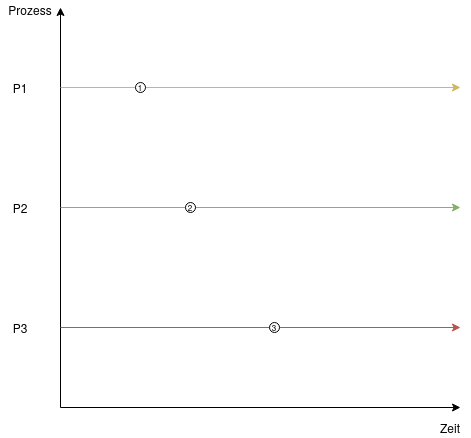
\includegraphics[width=.8\linewidth]{img/synchronisation/PartialOrdering_Concurrent.png}
		\caption[Abbildung]{Zeigt Prozesse P1, P2 und P3. Diese generieren jeweils ein Event.}
		\label{fig:Partial_Ordering_Concurrent_explained_1}
	\end{subfigure}
	\begin{subfigure}[t]{.49\linewidth}
		\centering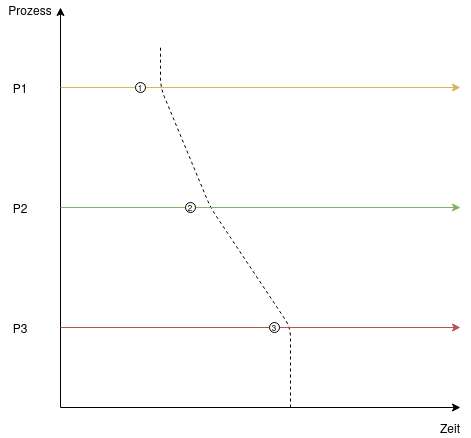
\includegraphics[width=.8\linewidth]{img/synchronisation/PartialOrdering_Concurrent_Explained}
		\caption[Abbildung]{Events (1), (2) und (3) finden parallel statt.}
		\label{fig:Partial_Ordering_Concurrent_explained_2}
	\end{subfigure}
\caption[Partielle Ordnung der Events dreier Prozesse]{}
\end{figure} 


Die \cref{fig:Partial_Ordering_Concurrent_explained_1} stellt eine Situation dar, in der drei Prozesse jeweils ein Event erzeugen. Intuitiv würde man interpretieren, dass (1) von P1 vor (2) von P2 erzeugt wurde und das darauf (3) von P3 folgt. Dies mag stimmen, in der Annahme, das es nur eine globale Zeit als richtwert gäbe. Allerdings lässt sich die Ordnung, in dem Kontext von verteilten Systemen und Nebenläufigkeit, nicht ohne Berücksichtignug verschiedener Einflussfaktoren feststellen. Lamport erläutert, dass in einer Umgebung, in der eine Ordnung anhand eines Zeitstempels physikalischer Zeit festgelegt wird, eine physikalische Uhr vorhanden sein muss.\footpartcite[S. 559]{lamport78} Die Einbindung einer physikalischen Uhr in ein verteiltes System ist eine aufwendige und komplexe Aufgabe. Probleme wie Synchronisation verschiedener Uhren mit keiner absoluten Präzision und dem dazugehörigen Drift, dem algorithmisch entgegengewirkt werden muss, treten auf. \cref{fig:Partial_Ordering_Concurrent_explained_2} zeigt, dass die Events, unter der Berücksichtigung der Definition von Lamport, nebenläufig stattfindet.  Aus diesem Grund ist es naheliegend zu versuche eine Lösung zu finden, die auf physikalische Uhren verzichtet.


Drei Bedingungen müssen nach Lamport erfüllt sein, damit eine Beziehung zwischen Events partiell geordnet ist. 
\begin{quote}
	\glqq (1) Wenn \emph{a} und \emph{b} Events im selben Prozess sind und \emph{a} vor \emph{b} stattfindet, dann \emph{a} $\rightarrow$ \emph{b}. (2) Wenn \emph{a} das Senden einer Nachricht eines Prozesses ist und \emph{b} das Empfangen einer Nachricht eines anderen Prozesses ist, dann \emph{a} $\rightarrow$ \emph{b}. (3) Wenn \emph{a} $\rightarrow$ \emph{b} und \emph{b} $\rightarrow$ \emph{c}, dann \emph{a} $\rightarrow$ \emph{c}.\grqq \:\footpartcite[S. 559]{lamport78}
\end{quote}

\begin{figure}[!ht]
	\centering
	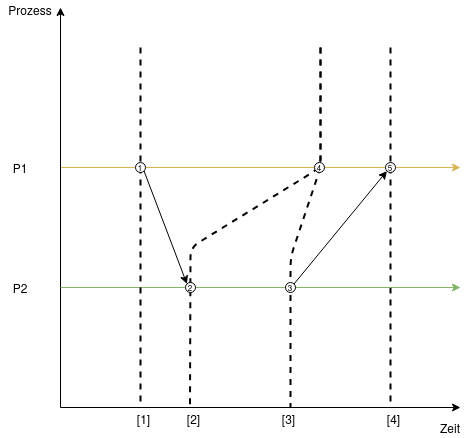
\includegraphics[scale=0.5]{img/synchronisation/PartialOrdering_ChildO.png}
	\caption[Partielle Ordnung von nebenläufigen Events]{Zeigt Prozesse P1 und P2. Diese generieren jeweils Events. Logische Reihenfolge des Auftretens der Events anhand der gestrichelten Linien [1], [2], [3] und [4] ersichtlich.}
	\label{fig:Partial_Ordering_Concurrent}
\end{figure}

Um die Feststellung von Lamport zu verdeutlichen wird \cref{fig:Partial_Ordering_Concurrent} untersucht. Die Abbildung stellt zwei Prozesse dar, dabei wird angenommen, dass diese in unterschiedlichen Rechensystemen angesiedelt sind. Das bedeutet, dass auf eine globale physikalische Uhr verzichtet wird. Diese Prozesse können sich mittels senden einer Nachricht und empfangen einer Nachricht verständigen. Das verteilte System generiert insgesamt fünf Events. P1 erzeugt (1) in der logischen Zeitspanne [1] und sendet anschließend eine Nachricht an P2. Das Empfangen wird durch (2) dargestellt. Daraus folgt, dass eine \emph{Happens Before Relation} zwischen (1) und (2) besteht, also (1) $\rightarrow$ (2). Nebenläufig dazu, findet in P1 Event (4) statt. (4) kann durch P2, in dieser Zeitspanne, in keiner Weise beeinflusst werden. Das heißt, dass (4) ein von (2)  kausal unabhängiges Ereignis ist, (2) $\not\rightarrow$ (4). (4) ist aber kausal von (1) abhängig, da es das direkt folgende Event im gleichen Prozess ist, also (1) $\rightarrow$ (4). (4) bildet dabei, als neues abhängiges Event, Zeitspanne [2]. Weitergehend zu folgern ist, (2) $\rightarrow$ (3), weshalb [3] entsteht. Auch hier ist eine kausale unabhängigkeit von (3) zu (4) zu sehen. An dieser Stelle spielt eine weitere Bedingung eine Rolle. Es muss die \emph{Clock Condition} berücksichtigt werden. Diese Bedingungen besagt:

\[
\text{Clock Condition}: \; \text{wenn} \; \emph{a} \rightarrow \emph{b} \; \text{dann} \; C(\emph{a})<C(\emph{b})
\]
Diese Bedingung führt $C$ als logische Uhr ein. Eine logische Uhr ist ein von der physikalischen Zeit unabhängiger Zähler, der einem Event eine Zahl zuweist. Die Clock Conditions ist erfüllt, sobald (1) darauf geachtet wird, dass zwischen zwei Events eines Prozesses die logische Uhr voranschreitet und (2) das einem Event ein Zeitstempel zugewiesen wird, der folgende Eigenschaften hat\footpartcite[S. 560]{lamport78}:
\[
 T_m = C_i \langle a \rangle \; 
 \text{dann} \; 
 {{C}_{j+1}} = \max[C_j,T_m]
\]
Dabei ist $T_m$ der Zeitstempel eines Events, welcher eine Nachricht $m$ zu einem anderen Prozess sendet, zum Zeitpunkt $C_i \langle a \rangle$. Beim empfangenen Prozess wird das erzeugte Event mit dem Zeitstempel ${{C}_{j+1}} = \max[C_j,T_m]$ versehen. Das bedeutet für die Darstellung, dass (3) $\not\rightarrow$ (4), (3) $\rightarrow$ (5) und $C_{P1} \langle 4 \rangle < C_{P2} \langle 3 \rangle$. Diese Annahme kann getroffen werden, weil (2)$\rightarrow$ (3) und somit diese beiden Events nicht zu einem Zeitpunkt mit (4) stattfinden können, weil es $C_{P2} \langle 2 \rangle < C_{P2} \langle 3 \rangle$ widersprechen würde.

 Die \textbf{Transitivität} ist durch (1) $\rightarrow$ (2) und (2) $\rightarrow$ (3) gegeben. Das heißt eine Relation zwischen (1) und (3) besteht, also (1) $\rightarrow$ (3). Die zweite Charakteristik, dass ein Event nicht vor sich selbst stattfinden kann, ist gegeben.(1) $\rightarrow$ (1) kann also nicht bestehen und ist somit \textbf{irreflexiv}. Zuletzt die ist durch die Tatsache, dass ein Event nicht vor und nach einem anderen parallel bestehen kann, also (1) $\rightarrow$ (2) und (2) $\rightarrow$ (1), gezeigt, dass die Relation \textbf{antisymmetrisch} ist. Die Kombination der drei Charakterisitken machen eine strikte partielle Ordnung aus, eine sogenannte Kausalordnung.

Die gezeigte Kausalordnung von Events stellt das Fundament zur Erhebung von Tracedaten in verteilten Systemen dar und ist somit unerlässlich, um ein verteiltes System beobachtbar zu machen, also einen Teil der \emph{Oberservability} zu ermöglichen.

\section{Distributed Tracing}
\label{subsection:Erkenntnisinteresse}
Der Begriff des Verteilte Systems wurden bereits nach Tanenbaum definiert. Allerdings lohnt es sich eine alternative Definition zu betrachten, die eine andere Perspektive ermöglicht. 

\begin{quote}
	Ein verteiltes System ist ein System, mit dem ich nicht arbeiten kann, weil irgendein Rechner abgestürzt ist, von dem ich nicht einmal weiß, dass es ihn überhaupt gibt.\footpartcite{lamport87}
\end{quote}


Diese Definition lässt sich so auffassen, dass Lamport im Jahr 1987 die Problematik der Fehlersuche während der Laufzeit, des Debuggings während der Entwicklungsphase und des organisatorischen Aufwands im Allgemeinen, also damit der grundsätzlich hohen Unübersichtlichkeit und Komplexität von verteilten Systemen, beschreibt. Diese Probleme und Herausforderungen, mit denen man in der heutigen Zeit der serviceorientierten Architektur beziehungsweise der Microservicearchitektur konfrontiert wird, können durch distributed tracing angegangen werden. So kann zum Beispiel Fehlerquellenermittlung beschleunigt werden. Tracing ist ein Konzept, welches als Werkzeug umgesetzt werden kann. Durch das Erheben von Tracedaten lassen sich detailierte Schlussfolgerungen über einzelne \emph{Requests} und ihren Weg durch das verteilte System schließen. Dies verlangt allerdings das direkte Eingreifen in den Quellcode. Der alternative Ansatz des \emph{Blackbox Monitoring}, also das Überwachen eines Systems mit eingeschränkten Informationen, wird in sich überschneidenden Anwendungsbereichen eingesetzt. Das Blackbox Monitoring versucht das System von Außen zu betrachten. Dabei wird keine Instrumentalisierung von Quellcode vorgenommen. Dieser sammelt Daten aus bestehenden Logs und Netzwerkschnittstellenüberwachung. Der Ansatz des Blackboxmonitoring ist sinnvoll, wenn mit vielen Softwarekomponenten gearbeitet wird, auf deren Entwicklung man keinen direkten Einfluss hat. Dazu zählen beispielsweise proparitäre Software, ohne Zugang zu dem Quellcode. Allerdings ist die Rekonstruktion der Requestpfade unzuverlässig und die Fehlerfreiheit, der gesamten Kausalordnung aller erzeugten Events, aufgrund der eingeschränkten Informationen, nicht ohne Nachteile, gegeben. 


Distributed tracing umfasst zwei Teilbereiche der im \cref{subsection:Beobachtbarkeit von verteilten Systemen} beschriebenen Beobobachtbarkeit von verteilten Systemen. Das ist zum einen die verteilte Anwendung mit ihren einzelnen Serviceskomponenten und zum anderen das Netzwerk über das Nachrichten ausgetauscht werden. In \cref{chapter:Problembeschreibung} wird anhand eines minimalbeispiels beschrieben, welche Rollen diese beiden Aspekte in der Generierung und Ordnung von Events zu spielen haben.

Ziel von distributed tracing soll sein, mit möglichst wenig \emph{overhead} und \emph{minimalem Aufwand} tiefgreifenden Einblick in eine verteilte Anwendung zu gewinnen. Mit wenig overhead ist gemeint, dass das System nicht zu stark beeinträchtigt wird. Das heißt, dass es zu keiner unvereantwortlichen Einbüßung von Leistung kommen darf. Das Bedürfnis nach minimalem Aufwand stammt von der Natur der Microservice-Architektur. Das Prinzip von loose gekoppelten und jederzeit austauschbaren Microservices fordert eine schnelle und einheitliche  Möglichkeit, Einblick in die Komplexität von verteilten Systemen zu gewinnnen. Dabei ist es erforderlich und aus Entwicklersicht verständlich, dass der Instrumentalisierungsanteil des Services nur ein kleinen Teil der Gesamtlogik ausmachen darf. Den die Entwickler wollen sich auf die Businesslogik konzentrieren und distributed tracing soll den Entwicklungsprozess unterstützen und nicht durch übermäßige Investitionsanforderungen beeinträchtigen.

 
\section{Bibliotheksentwicklung}
\label{subsection:Bibliotheksentwicklung}

Das Konzept von \emph{distributed tracing} ist als Bibliothek in der Programmiersprache C\# umgesetzt. Die Auswahl der Sprache ergibt sich aus dem Anwendungsbereich. Aufgrund der Anforderung, dass eine einfache Integration in bereits bestehende Projekte wünschenswert ist, wird die Bilbiothek über den Packetmanager \emph{Nuget} veröffentlicht. Dies ermöglicht in den Entwicklungsumgebungen wie zum Beispiel \emph{Unity} auf Linux wie auch auf Windows eine einfache und schnelle integration. Durch den Entwicklungsprozess ist eine \gls{ciGlossar} Pipeline aufgebaut worden. 

\begin{itemize}
	\item c\# 
	\item tracing kozept als bibliothek umgesetzt
	\item bereitstellung über packetmanager nuget
	\item weil entwicklungsumgebung windows als auch linux 
\end{itemize} 
% ----------------------------------------------------------------------------
